\documentclass{exam}
\usepackage{main}
\title{Evaluation de Cours}
\date{11 Décembre 2023}

\qformatExos
\begin{document}
\maketitle
\begin{questions}
\question Soit une fonction $f$ définie sur $[-2;5]$, et dont la courbe représentative est donnée ci-dessous.
\begin{center}
\begin{tikzpicture}
\shorthandoff{:}
\millirepere[step=0.5](-2.25,-4.25) -- (5.25, 4.25);
\draw[thick] (1,-0.25) -- (1,0.25) node[left] {$1$};
\draw[thick] (-0.25,1) -- (0.25,1) node[above] {$1$};
\draw[domain=-2:5] plot (\x, {(\x + 1)*(\x - 3)/4});
\end{tikzpicture}
\end{center}
\begin{parts}
\vspace{0.5cm}
\part Compléter le tableau de signe ci-dessous :
\begin{center}
\begin{tikzpicture}
\tkzTabInit{$x$ / 1, $f(x)$ / 1}{$-2$, $\dots$, $\dots$, $5$}
\tkzTabLine{,$\dots$,z,$\dots$,z,$\dots$}
\end{tikzpicture}
\end{center}
\vspace{0.5cm}
\part En déduire sur quel ensemble la fonction $f$ est positive, c'est-à-dire trouver les solutions de $f(x) \geq 0$. Indication : utiliser une réunion d'intervalles.
\end{parts}
\end{questions}
\end{document}
